\documentclass{exam}

\usepackage{units} 
\usepackage{graphicx}
\usepackage[fleqn]{amsmath}
\usepackage{cancel}
\usepackage{float}
\usepackage{mdwlist}
\usepackage{booktabs}
\usepackage{cancel}
\usepackage{polynom}
\usepackage{caption}
\usepackage{fullpage}
\usepackage{xfrac}
\usepackage{enumerate}

\newcommand{\dg}{\ensuremath{^\circ}} 
\everymath{\displaystyle}

\printanswers

\title{Math 142 Notes \\ Section 7.3}

\date{\today}

\begin{document}

  \maketitle
  \tableofcontents

  \section{Double Angle Formulas}

  \subsection{$\cos 2x$}
  \begin{align*}
    \cos(x + x) & = \cos x \cos x - \sin x \sin x \\
    \cos 2x     & = \cos^2 x - \sin^2 x \\
                & = 1 - 2 \sin^2 x \\
                & = 2 \cos^2 x - 1 \\
  \end{align*}

  \subsection{$\sin 2s$}
  \begin{align*}
    \sin(x + x) & = \sin x \cos x + \cos x \sin x \\
    \sin 2x     & = 2 \cos x \sin x \\
  \end{align*}

  \subsection{$\tan 2s$}
  \begin{align*}
    \tan 2x & = \frac{\sin 2x}{\cos 2x} \\
            & = \frac{2 \cos x \sin x}{\cos^2 x - \sin^2 x} \\
            & = \frac{2 \cos x \sin x}{\cos^2 x - \sin^2 x} \cdot \frac{\sfrac{1}{\cos^2 x}}{\sfrac{1}{\cos^2 x}} \\
            & = \frac{2 \tan x}{1 - \tan^2 x} \\
  \end{align*}

  \section{Power Lowering Formulas}

  \subsection{$\sin^2 s$}
  \begin{align*}
    \cos 2x  & = 1 - 2 \sin^2 x \\
    \sin^2 x & = \frac{1 - \cos 2x}{2} \\
  \end{align*}

  \subsection{$\cos^2 x$}
  \begin{align*}
    \cos 2x  & = 2 \cos^2 x - 1 \\
    \cos^2 x & = \frac{1 + \cos 2x}{2} \\
  \end{align*}

  \subsection{$\tan^2 s$}
  \[
    \tan^2 x = \frac{1 - \cos 2x}{1 + \cos 2x}
  \]

  \section{Half Angle Formulas}

  \subsection{$\sin \sfrac{x}{2}$}
  \begin{align*}
    \sin^2 x         & = \frac{1 - \cos 2x}{2} \\
    \sin x           & = \pm \sqrt{ \frac{1 - \cos 2x}{2} } \\
    \sin \frac{x}{2} & = \pm \sqrt{ \frac{1 - \cos x}{2} } \\
  \end{align*}

  \subsection{$\cos \sfrac{x}{2}$}
  \begin{align*}
    \cos^2 x         & = \frac{1 + \cos 2x}{2} \\
    \cos x           & = \pm \sqrt{ \frac{1 + \cos 2x}{2} } \\
    \cos \frac{x}{2} & = \pm \sqrt{ \frac{1 + \cos x}{2} } \\
  \end{align*}

  \subsection{$\tan \sfrac{x}{2}$}
  \begin{align*}
    \tan^2 x           & = \frac{1 - \cos 2x}{1 + \cos 2x} \\
    \tan^2 \frac{x}{2} & = \frac{1 - \cos x}{1 + \cos x} \\
    \tan \frac{x}{2}   & = \pm \sqrt{ \frac{1 - \cos x}{1 + \cos x} } \\
                       & = \pm \sqrt{ \frac{1 - \cos x}{1 + \cos x} \cdot \frac{1 - \cos x}{1 - \cos x} } \\
                       & = \pm \sqrt{ \frac{(1 - \cos x)^2}{1 - \cos^2 x} } \\
                       & = \pm \sqrt{ \frac{(1 - \cos x)^2}{\sin^2 x} } \\
                       & = \pm \left| \frac{1 - \cos x}{\sin x} \right| \\
                       & = \frac{1 - \cos x}{\sin x} \\
  \end{align*}

  $\sin x$ and $\tan \sfrac{x}{2}$ always have the same sign.

  \begin{align*}
    \sin 2x          & = 2 \sin x \cos x \\
    \sin x           & = 2 \sin \frac{x}{2} \cos \frac{x}{2} \\
    \tan \frac{x}{2} & = \frac{\sin \sfrac{x}{2}}{\cos \sfrac{x}{2}} \\
  \end{align*}

  \begin{figure}[H]
    \centering
    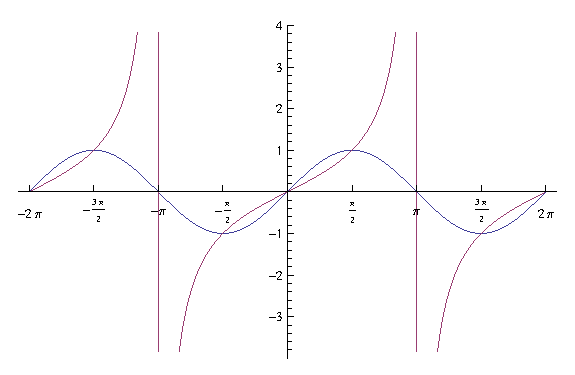
\includegraphics[scale=0.8]{sinx_tanx2}
    \caption{$sin x$ and $tan \sfrac{x}{2}$}
  \end{figure}

\end{document}
